% Asset ID: AS1VectorsTikZ-003
% Source: P1-Chp11-Vectors.pdf, Representing Vectors slide
% Related lesson section: Key Definitions and Notation; Core Theory: Component form and i,j form
% Purpose: Show column vector components and i,j basis vectors.
\documentclass[tikz,border=8pt]{standalone}
\usepackage{amsmath}
\usepackage{bm}
\usetikzlibrary{arrows.meta,positioning,angles,quotes}
\begin{document}

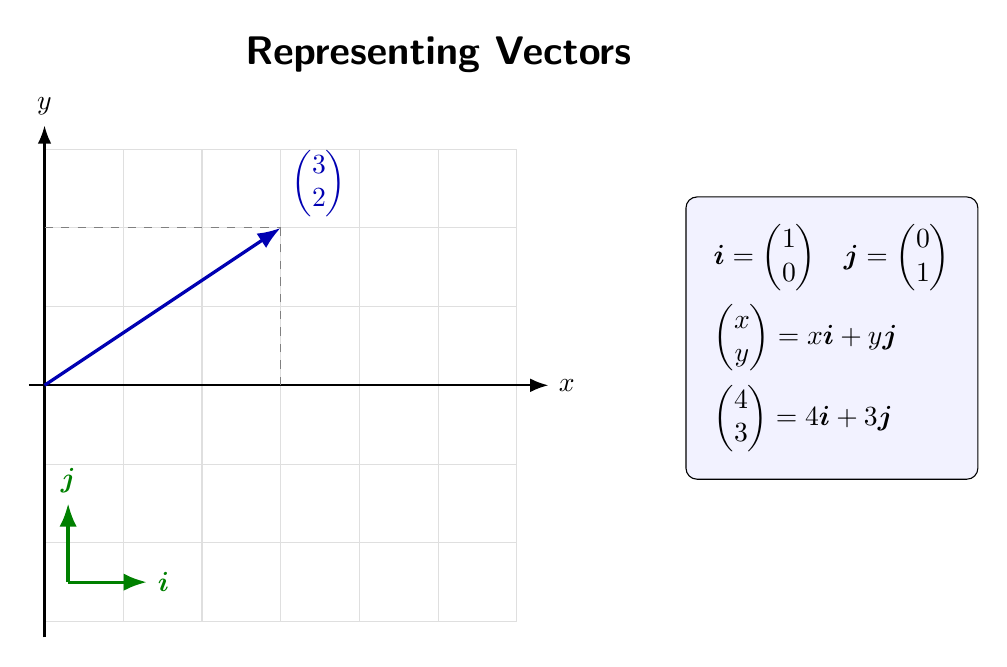
\begin{tikzpicture}[>=Latex,every node/.style={font=\sffamily},vector/.style={->,very thick,blue!70!black},basis/.style={->,very thick,green!50!black}]
\node[font=\sffamily\bfseries\Large] at (0,4.2) {Representing Vectors};
\draw[step=1,gray!25] (-5,-3) grid (1,3);\draw[->,thick] (-5.2,0)--(1.4,0) node[right] {$x$};\draw[->,thick] (-5,-3.2)--(-5,3.3) node[above] {$y$};
\draw[vector] (-5,0)--(-2,2) node[above right] {$\begin{pmatrix}3\\2\end{pmatrix}$};
\draw[dashed,gray] (-2,0)--(-2,2);\draw[dashed,gray] (-5,2)--(-2,2);
\draw[basis] (-4.7,-2.5)--(-3.7,-2.5) node[right] {$\bm i$};\draw[basis] (-4.7,-2.5)--(-4.7,-1.5) node[above] {$\bm j$};
\node[draw,rounded corners,fill=blue!5,align=left,inner sep=10pt] at (5,0.6) {$\bm i=\begin{pmatrix}1\\0\end{pmatrix}$\quad $\bm j=\begin{pmatrix}0\\1\end{pmatrix}$\\[4pt]$\begin{pmatrix}x\\y\end{pmatrix}=x\bm i+y\bm j$\\[4pt]$\begin{pmatrix}4\\3\end{pmatrix}=4\bm i+3\bm j$};
\end{tikzpicture}

\end{document}
